%LaTex cheat sheet template
\documentclass[10pt,a4paper,landscape]{article}

\usepackage{xfrac}
\usepackage[utf8]{inputenc}
\usepackage{amsmath}
\usepackage{amsfonts}
\usepackage{amssymb}
\usepackage{multicol}
\usepackage{geometry}
\usepackage{lipsum}
\usepackage{titlesec}
\usepackage[nodisplayskipstretch]{setspace}

\geometry{a4paper, total={297mm,210mm}, left=2mm, top=0mm, right=0mm, bottom=3mm}

\titlespacing{\section}{0pt}{0pt}{0pt}
\titlespacing{\subsection}{0pt}{0pt}{0pt}
\titlespacing{\subsubsection}{0pt}{0pt}{0pt}


% \setlength{\abovedisplayskip}{0pt}
% \setlength{\belowdisplayskip}{0pt}

\begin{document}
\begin{multicols*}{3}
    \section*{Formulaire CompAlg}
    \subsection*{Équations différentielles}
\noindent
$h$ : pas de discrétisation\\
Il faut isoler $y^{\prime}$ tel que $y^{\prime}=f(t,y)$
\subsubsection*{Euler (un étage)}
\noindent
\begin{equation}
    \left\{
    \begin{aligned}
        y_{n+1} & = y_n + h\cdot f(t_n, y_n), \\
        t_{n+1} & = t_n + h
    \end{aligned}
    \right.
    \nonumber
\end{equation}
\subsubsection*{Point milieu}
\noindent
\begin{equation}
    \left\{
    \begin{aligned}
         & s_1     = f(t_n,y_n),                                             \\
         & s_2     = f\left(t_n+\frac{h}{2},y_n+\frac{h}{2}\cdot s_1\right), \\
         & y_{n+1} = y_n+h\cdot s_2,                                         \\
         & t_{n+1} = t_n+h.
    \end{aligned}
    \right.
    \nonumber
\end{equation}
\subsubsection*{Trapèze}
\noindent
\begin{equation}
    \left\{
    \begin{aligned}
         & s_1     = f(t_n,y_n),                         \\
         & s_2     = f\left(t_n+h,y_n+h\cdot s_1\right), \\
         & y_{n+1} = y_n+\frac{h}{2}\cdot(s_1+s_2),      \\
         & t_{n+1} = t_n+h.
    \end{aligned}
    \right.
    \nonumber
\end{equation}
\subsubsection*{Runge-Kutta d'ordre 2 (forme générale)}
\noindent
\begin{equation}
    \left\{
    \begin{aligned}
         & s_1     = f(t_n,y_n),                                              \\
         & s_2     = f\left(t_n+c_2\cdot h,y_n+a_{21}\cdot h\cdot s_1\right), \\
         & y_{n+1} = y_n+h\cdot (\omega_1\cdot s_1 + \omega_2\cdot s_2),      \\
         & t_{n+1} = t_n+h.
    \end{aligned}
    \right.
    \nonumber
\end{equation}
Il est possible de représenter les différents paramètres intervenant dans une méthode
de Runge-Kutta d'ordre 2 ($c_2$, $a_21$, $w_1$ et $w_2$) dans un tableau
\begin{center}
    \begin{tabular}{c|c c}
        0     &            &            \\
        $c_2$ & $a_{21}$                \\
        \hline
              & $\omega_1$ & $\omega_2$
    \end{tabular}
\end{center}
point milieu (droite), optimal (milieu), trapèze (gauche)
\begin{center}
    \begin{tabular}{c|c c}
        0              &                &   \\
        $\sfrac{1}{2}$ & $\sfrac{1}{2}$ &   \\
        \hline
                       & 0              & 1
    \end{tabular}
    \begin{tabular}{c|c c}
        0              &                &                \\
        $\sfrac{2}{3}$ & $\sfrac{2}{3}$ &                \\
        \hline
                       & $\sfrac{1}{4}$ & $\sfrac{3}{4}$
    \end{tabular}
    \begin{tabular}{c|c c}
        0 &                &                \\
        1 & 1              &                \\
        \hline
          & $\sfrac{1}{2}$ & $\sfrac{1}{2}$
    \end{tabular}
\end{center}
\subsubsection*{Runge-Kutta d'ordre 3 (forme générale)}
\noindent
\begin{equation}
    \left\{
    \begin{aligned}
         & s_1     = f(t_n,y_n),                                                                     \\
         & s_2     = f\left(t_n+c_2\cdot h,y_n+a_{21}\cdot h\cdot s_1\right),                        \\
         & s_3     = f\left(t_n+c_3\cdot h,y_n+a_{31}\cdot h\cdot s_1+a_{32}\cdot h\cdot s_2\right), \\
         & y_{n+1} = y_n+h\cdot (\omega_1\cdot s_1 + \omega_2\cdot s_2 + \omega_3\cdot s_3),         \\
         & t_{n+1} = t_n+h.
    \end{aligned}
    \right.
    \nonumber
\end{equation}
Kutta (droite), $\sfrac{2}{3}$ (milieu), optimale (gauche)
\begin{center}
    \begin{tabular}{c|c c c}
        0              &                &                &                \\
        $\sfrac{1}{2}$ & $\sfrac{1}{2}$ &                &                \\
        1              & $-1$           & 2              &                \\
        \hline
                       & $\sfrac{1}{6}$ & $\sfrac{2}{3}$ & $\sfrac{1}{6}$
    \end{tabular}
    \begin{tabular}{c|c c c}
        0              &                &                &                \\
        $\sfrac{1}{2}$ & $\sfrac{1}{2}$ &                &                \\
        $\sfrac{3}{4}$ & 0              & $\sfrac{3}{4}$ &                \\
        \hline
                       & $\sfrac{2}{9}$ & $\sfrac{3}{9}$ & $\sfrac{4}{9}$
    \end{tabular}
    \begin{tabular}{c|c c c}
        0              &                &                &                \\
        $\sfrac{2}{3}$ & $\sfrac{2}{3}$ &                &                \\
        $\sfrac{2}{3}$ & $\sfrac{1}{3}$ & $\sfrac{1}{3}$ &                \\
        \hline
                       & $\sfrac{1}{4}$ & 0              & $\sfrac{3}{4}$
    \end{tabular}
\end{center}
\subsubsection*{Runge-Kutta classique}
\noindent
\begin{equation}
    \left\{
    \begin{aligned}
         & s_1     = f(t_n,y_n),                                             \\
         & s_2     = f\left(t_n+\frac{h}{2},y_n+\frac{h}{2}\cdot s_1\right), \\
         & s_3     = f\left(t_n+\frac{h}{2},y_n+\frac{h}{2}\cdot s_2\right), \\
         & s_4     = f(t_n+h,y_n+h\cdot s_3),                                \\
         & y_{n+1} = y_n+\frac{h}{6}\cdot(s_1+2\cdot s_2+2\cdot s_3+s_4),    \\
         & t_{n+1} = t_n+h.
    \end{aligned}
    \right.
    \nonumber
\end{equation}
\subsubsection*{Runge-Kutta-Fehlberg}
\noindent
\begin{equation}
    \left\{
    \begin{aligned}
         & s_1     = f(t_n,y_n),                                                           \\
         & s_2     = f\left(t_n+\frac{h}{2},y_n+\frac{h}{2}\cdot s_1\right),               \\
         & s_3     = f\left(t_n+\frac{3}{4}\cdot h,y_n+\frac{3}{4}\cdot h\cdot s_2\right), \\
         & y_{n+1} = y_n+\frac{h}{9}\cdot(2\cdot s_1+3\cdot s_2+4\cdot s_3),               \\
         & s_4     = f(t_n+h,y_{n+1}),                                                     \\
         & e_{n+1} = \frac{h}{72}\cdot(-5\cdot s_1+6\cdot s_2+8\cdot s_3-9\cdot s_4),      \\
         & t_{n+1} = t_n+h.
    \end{aligned}
    \right.
    \nonumber
\end{equation}
\subsubsection*{Systèmes d'équations différentielles}
\noindent
On peut transformer une équation différentielle d'ordre $n$ en un système d'équations
différentielles d'ordre 1. Au lieu d'avoir $n$ dérivées, on a $n$ fonctions inconnues.\\
\textbf{Exemple :} $x^{\prime\prime}(t)=-\sin(t)\cdot x^\prime(t)+2\cdot x(t)$
\begin{equation}
    \begin{gathered}
        \begin{array}{cc}
            y(t)=\begin{pmatrix} x \\ x' \end{pmatrix}, & y^\prime(t) = \begin{pmatrix} x' \\ x'' \end{pmatrix} = \begin{pmatrix} x' \\ -\sin(t)\cdot x^\prime+2\cdot x \end{pmatrix},
        \end{array} \\
        y^\prime\left(t,\binom{y_1}{y_2}\right)=\binom{y_2}{-\sin(t)\cdot y_2+2\cdot y_1}
    \end{gathered}
    \nonumber
\end{equation}
Ensuite, on peut appliquer une méthode numérique à ce système d'équations différentielles.
On aura donc, par exemple pour Euler :
\begin{equation}
    \left\{
    \begin{aligned}
         & y_{1,n+1} = y_{1,n} + h\cdot y_{2,n},                                  \\
         & y_{2,n+1} = y_{2,n} + h\cdot (-\sin(t_n)\cdot y_{2,n}+2\cdot y_{1,n}), \\
         & t_{n+1} = t_n + h.
    \end{aligned}
    \right.
    \nonumber
\end{equation}
Et pour une méthode de Runge-Kutta on devrait calculer deux $s_1$, $s_2$, etc.
et pour chaque pas de temps $t_n$ on aura deux valeurs $y_{1,n}$ et $y_{2,n}$.
    \newpage
    \subsection*{Algèbre linéaire numérique}
\noindent
On peut réécrire un système d'équations linéaires sous la forme $A\cdot x=b$.
\begin{equation}
    \begin{pmatrix}
        a_{11} & a_{12} & \cdots & a_{1n} \\
        a_{21} & a_{22} & \cdots & a_{2n} \\
        \vdots & \vdots & \ddots & \vdots \\
        a_{m1} & a_{m2} & \cdots & a_{mn}
    \end{pmatrix}
    \cdot
    \begin{pmatrix}
        x_1    \\
        x_2    \\
        \vdots \\
        x_n
    \end{pmatrix}
    =
    \begin{pmatrix}
        b_1    \\
        b_2    \\
        \vdots \\
        b_m
    \end{pmatrix}
    \nonumber
\end{equation}
Pour les exemples on prend toujours le système suivant :
\begin{equation}
    \begin{pmatrix}
        1 & 2 & 3 \\
        4 & 5 & 6 \\
        7 & 8 & 9
    \end{pmatrix}
    \cdot
    \begin{pmatrix}
        x_1 \\
        x_2 \\
        x_3
    \end{pmatrix}
    =
    \begin{pmatrix}
        1 \\
        2 \\
        3
    \end{pmatrix}
    \nonumber
\end{equation}
\subsubsection*{Méthode de Gauss}
\noindent
\begin{equation}
    \left(\begin{array}{ccc|c}
        1 & 2 & 3 & 1 \\
        4 & 5 & 6 & 2 \\
        7 & 8 & 9 & 3
    \end{array}\right)
    \rightarrow
    \left(\begin{array}{ccc|c}
        1 & 2  & 3   & 1  \\
        4 & 4  & 6   & 2  \\
        0 & -6 & -12 & -4
    \end{array}\right)
    \nonumber
\end{equation}
\begin{equation}
    \rightarrow
    \left(\begin{array}{ccc|c}
        1 & 2 & 3  & 1  \\
        4 & 5 & 6  & 2  \\
        0 & 0 & -3 & -1
    \end{array}\right)
    \rightarrow
    \left(\begin{array}{ccc|c}
        1 & 2  & 3  & 1  \\
        0 & -3 & -6 & -2 \\
        0 & 0  & -3 & -1
    \end{array}\right)
    \nonumber
\end{equation}
Puis on remonte et on trouve $x_3=\sfrac{-4}{-6}=\sfrac{2}{3}$, $x_2=\dots$
\subsubsection*{Décomposition LU}
\noindent
Le but de la décomposition LU est de factoriser la matrice $A$ en
deux matrices $L$ et $U$ telles que $A=L\cdot U$. Elle ne s'applique qu'aux
matrices carrées.\\
\begin{equation}
    \begin{pmatrix}
        a_{11} & a_{12} & a_{13} \\
        a_{21} & a_{22} & a_{23} \\
        a_{31} & a_{32} & a_{33}
    \end{pmatrix}
    =
    \begin{pmatrix}
        1      & 0      & 0 \\
        l_{21} & 1      & 0 \\
        l_{31} & l_{32} & 1
    \end{pmatrix}
    \cdot
    \begin{pmatrix}
        u_{11} & u_{12} & u_{13} \\
        0      & u_{22} & u_{23} \\
        0      & 0      & u_{33}
    \end{pmatrix}
    \nonumber
\end{equation}
Les coefficients sont calculés comme suit :
\begin{equation}
    \begin{aligned}
         & a_{11}= 1 \cdot u_{11} + 0 \cdot 0 + 0 \cdot 0           \\
         & a_{12}= 1 \cdot u_{12} + 0 \cdot u_{22} + 0 \cdot 0      \\
         & a_{13}= 1 \cdot u_{13} + 0 \cdot u_{23} + 0 \cdot u_{33} \\
         & a_{21}= l_{21} \cdot u_{11} + 1 \cdot 0 + 0 \cdot 0      \\
         & a_{22}= l_{21} \cdot u_{12} + 1 \cdot u_{22} + 0 \cdot 0 \\
         & \dots
    \end{aligned}
    \nonumber
\end{equation}
Puis comme on connait les $a_{ij}$ on peut trouver les $l_{ij}$ et les $u_{ij}$.
Ensuite on résout le système $L\cdot \overrightarrow{y}=\overrightarrow{b}$ et
$U\cdot \overrightarrow{x}=\overrightarrow{y}$ :
\begin{equation}
    \begin{pmatrix}
        1      & 0      & 0 \\
        l_{21} & 1      & 0 \\
        l_{31} & l_{32} & 1
    \end{pmatrix}
    \cdot
    \begin{pmatrix}
        y_1 \\
        y_2 \\
        y_3
    \end{pmatrix}
    =
    \begin{pmatrix}
        1 \\
        2 \\
        3
    \end{pmatrix}
    \nonumber
\end{equation}
\begin{equation}
    \begin{pmatrix}
        u_{11} & u_{12} & u_{13} \\
        0      & u_{22} & u_{23} \\
        0      & 0      & u_{33}
    \end{pmatrix}
    \cdot
    \begin{pmatrix}
        x_1 \\
        x_2 \\
        x_3
    \end{pmatrix}
    =
    \begin{pmatrix}
        y_1 \\
        y_2 \\
        y_3
    \end{pmatrix}
    \nonumber
\end{equation}
Il faut faire attention si la première valeur de la matrice est très petite,
il faut permuter les lignes. Sinon, on peut avoir des erreurs d'arrondi à cause
des chiffres significatifs. 3 chiffres dans la mantisse signifie
: $1.234\cdot 10^6=1.230\cdot 10^6$\\
Attention si on permute des lignes, il faut aussi permuter les valeurs de $b$ :
\begin{equation}
    PA\overrightarrow{x}=P\overrightarrow{b}
    \nonumber
\end{equation}
\begin{equation}
    L\underbrace{U\overrightarrow{x}}_{\overrightarrow{y}}=P\overrightarrow{b}
    \nonumber
\end{equation}
\subsubsection*{Transformation de Householder}
\noindent
La transformation de Householder permet de transformer une matrice $A$ en une
matrice $R$ triangulaire supérieure. Pour cela il faut recalculer les vecteurs
$\overrightarrow{x}$ et les matrices $H$ pour chaque colonne de la matrice $A$.
\begin{equation}
    H\cdot \overrightarrow{x}=-\rho\cdot \overrightarrow{e}_1
    \nonumber
\end{equation}
Pour une matrice 3x3 :
\begin{equation}
    \begin{tabular}{cc}
        $\overrightarrow{x_1}=
            \begin{pmatrix}
                x_1 \\
                x_2 \\
                x_3
            \end{pmatrix}
            \rightarrow
        \begin{pmatrix}
                -\rho_1 \\
                0       \\
                0
            \end{pmatrix}$ &
        $\overrightarrow{x_2}=
            \begin{pmatrix}
                x_1 \\
                x_2 \\
                x_3
            \end{pmatrix}
            \rightarrow
            \begin{pmatrix}
                \alpha  \\
                -\rho_2 \\
                0
            \end{pmatrix}$
    \end{tabular}
    \nonumber
\end{equation}
\begin{equation}
    \overrightarrow{x_3}=
    \begin{pmatrix}
        x_1 \\
        x_2 \\
        x_3
    \end{pmatrix}
    \rightarrow
    \begin{pmatrix}
        \beta  \\
        \gamma \\
        \delta
    \end{pmatrix}
    \nonumber
\end{equation}
\begin{equation}
    \rho = \text{sign}(x_1)\cdot \left \|  \overrightarrow{x}\right \|_2
    \nonumber
\end{equation}
\begin{equation}
    \overrightarrow{v} = \overrightarrow{x}+\rho\cdot \overrightarrow{e}_1
    \nonumber
\end{equation}
\begin{equation}
    \gamma = \frac{\left \| \overrightarrow{v} \right \|_2^2}{2}=\rho\cdot v_1
    \nonumber
\end{equation}
Et donc la matrice $H$ se calcul :
\begin{equation}
    H=I-\frac{\overrightarrow{v}\cdot \overrightarrow{v}^T}{\gamma}
    \nonumber
\end{equation}
\subsubsection*{Décomposition QR}
\noindent
Le but de la décomposition QR est de factoriser la matrice $A$ en
deux matrices $Q$ et $R$ telles que $A=Q\cdot R$. Elle s'applique à toutes les
matrices.\\
Exemple pour une matrice 3x3 :\\
\textbf{1ère colonne :}
calculer $H_1$ avec $\overrightarrow{x_1}$ puis :
\begin{equation}
    A_1=H_1\cdot A = \begin{pmatrix}
        -\rho_1 & \alpha & \beta \\
        0       & \star  & \star \\
        0       & \star  & \star
    \end{pmatrix}
    \nonumber
\end{equation}
\textbf{2ère colonne :}
calculer $H_2$ avec $\overrightarrow{x_2}$ puis :
\begin{equation}
    A_2=H_2\cdot A_1 = \begin{pmatrix}
        -\rho_1 & \alpha  & \beta  \\
        0       & -\rho_2 & \gamma \\
        0       & 0       & \delta
    \end{pmatrix}
    \nonumber
\end{equation}
$H_2$ devrait être de la forme :
\begin{equation}
    H_2=\begin{pmatrix}
        1 & 0     & 0     \\
        0 & \star & \star \\
        0 & \star & \star
    \end{pmatrix}
    \nonumber
\end{equation}
\textbf{Résoudre le système :}
\begin{equation}
    Q^T = H_2\cdot H_1
    \nonumber
\end{equation}
\begin{equation}
    R = A_2
    \nonumber
\end{equation}
\begin{equation}
    \begin{tabular}{ccc}
        $R\cdot \overrightarrow{x}=Q^T\cdot \overrightarrow{b}$
         & $\Longleftrightarrow $
         & $A_2\cdot \overrightarrow{x}=H_2\cdot H_1\cdot \overrightarrow{b}$
    \end{tabular}
    \nonumber
\end{equation}
\subsubsection*{Méthode de Jacobi}
\noindent
Pour les méthodes itératives, il faut que la matrice soit diagonalement dominante :
\begin{equation}
    \left | a_{ii} \right | > \sum_{j=1,j\neq i}^{n} \left | a_{ij} \right |
    \nonumber
\end{equation}
Soit le système :
\begin{equation}
    \begin{pmatrix}
        10 & 1  \\
        2  & 10 \\
    \end{pmatrix}
    \cdot
    \begin{pmatrix}
        x_1 \\
        x_2
    \end{pmatrix}
    =
    \begin{pmatrix}
        11 \\
        12 \\
    \end{pmatrix}
    \nonumber
\end{equation}
Qu'on réécrit sous la forme :
\begin{equation}
    \left\{\begin{aligned}
         & 10\cdot x_1^{(k+1)}=-1\cdot x_2^{(k)}+11 \\
         & 10\cdot x_2^{(k+1)}=-2\cdot x_1^{(k)}+12
    \end{aligned}\right.
    \nonumber
\end{equation}
\begin{equation}
    \left\{\begin{aligned}
         & x_1^{(k+1)}=\frac{1}{10}\cdot(-1\cdot x_2^{(k)}+11) \\
         & x_2^{(k+1)}=\frac{1}{10}\cdot(-2\cdot x_1^{(k)}+12)
    \end{aligned}\right.
    \nonumber
\end{equation}
Pour estimer le nombre d'itérations à effectuer afin de réduire l'erreur initiale
d'un facteur $\tau$ il faut calculer le rayon spectral de la matrice d'itération
$E=I-NA$, dans le cas de la méthode de Jacobi :
\begin{equation}
    \varrho(E)=\max_i\left |\lambda_i(E) \right |
    \nonumber
\end{equation}
\begin{equation}
    E=I-D^{-1}\cdot A
    \nonumber
\end{equation}
\begin{equation}
    n \geq \frac{\ln(\tau)}{\ln(\varrho(E))}
    \nonumber
\end{equation}
\subsubsection*{Méthode de Gauss-Seidel}
\noindent
Même chose que pour la méthode de Jacobi, mais on utilise les nouvelles valeurs
dans la même itération :
\begin{equation}
    \left\{\begin{aligned}
         & x_1^{(k+1)}=\frac{1}{10}\cdot(-1\cdot x_2^{(k)}+11)   \\
         & x_2^{(k+1)}=\frac{1}{10}\cdot(-2\cdot x_1^{(k+1)}+12)
    \end{aligned}\right.
    \nonumber
\end{equation}
Matrice d'itérations pour réduire l'erreur initiale d'un facteur $\tau$ :
\begin{equation}
    E = I-(D+L)^{-1}\cdot A
    \nonumber
\end{equation}
\subsubsection*{Méthode de relaxation}
\noindent
Même chose que pour la méthode de Gauss-Seidel, mais on rajoute un poids $\omega$ :
\begin{equation}
    \left\{\begin{aligned}
         & x_1^{(k+1)}=(1-\omega)\cdot x_1^{(k)}+\frac{\omega}{10}\cdot(-1\cdot x_2^{(k)}+11)   \\
         & x_2^{(k+1)}=(1-\omega)\cdot x_2^{(k)}+\frac{\omega}{10}\cdot(-2\cdot x_1^{(k+1)}+12)
    \end{aligned}\right.
    \nonumber
\end{equation}
\subsubsection*{Méthode de descente pour \boldmath{$F(\overrightarrow{x})=\left \| \overrightarrow{b}-A \overrightarrow{x} \right \|_2^2$}}
\noindent
On veut minimiser la fonction $F(\overrightarrow{x})$.\\
$\overrightarrow{x_0}$ étant le vecteur de départ (aléatoire), on calcule :\\
\textbf{L'erreur}
\begin{equation}
    F(\overrightarrow{x_0})=\left \| \overrightarrow{b}-A\cdot \overrightarrow{x_0} \right \|_2^2
    \nonumber
\end{equation}
\textbf{Le résidu}
\begin{equation}
    \overrightarrow{r_0}=\overrightarrow{b}-A\cdot \overrightarrow{x_0}
    \nonumber
\end{equation}
\textbf{Le gradient de \boldmath{$F(\overrightarrow{x})$}}
\begin{equation}
    \nabla F(\overrightarrow{x_0})=-2\cdot A^T\cdot \overrightarrow{r_0}
    \nonumber
\end{equation}
\textbf{La direction de descente}
\begin{equation}
    \overrightarrow{d_0}=-\nabla F(\overrightarrow{x_0})=2\cdot A^T\cdot \overrightarrow{r_0}
    \nonumber
\end{equation}
\textbf{Le pas}
\begin{equation}
    \alpha_0=\frac{\overrightarrow{r_0}^T\cdot A\cdot \overrightarrow{d_0}}{\overrightarrow{d_0}^T\cdot A^T\cdot A\cdot \overrightarrow{d_0}}
    \nonumber
\end{equation}
\textbf{Le nouveau vecteur}
\begin{equation}
    \overrightarrow{x_1}=\overrightarrow{x_0}+\alpha_0\cdot \overrightarrow{d_0}
    \nonumber
\end{equation}
Puis recommencer pour $\overrightarrow{x_1}$, $\overrightarrow{x_2}$, $\dots$\\
\subsubsection*{Méthode de descente pour \boldmath{$G(\overrightarrow{x})=\frac{1}{2} \overrightarrow{x}^T A \overrightarrow{x}-\overrightarrow{x}^T\overrightarrow{b}$}}
\noindent
On veut minimiser la fonction $G(\overrightarrow{x})$.\\
$\overrightarrow{x_0}$ étant le vecteur de départ (aléatoire), on calcule :\\
\textbf{L'erreur}
\begin{equation}
    G(\overrightarrow{x_0})=\frac{1}{2}\cdot \overrightarrow{x_0}^T\cdot A\cdot \overrightarrow{x_0}-\overrightarrow{x_0}^T\cdot \overrightarrow{b}
    \nonumber
\end{equation}
\textbf{Le gradient de \boldmath{$G(\overrightarrow{x})$}}
\begin{equation}
    \nabla G(\overrightarrow{x_0})=A\cdot \overrightarrow{x_0}-\overrightarrow{b}
    \nonumber
\end{equation}
\textbf{Le résidu et la direction de descente}
\begin{equation}
    \overrightarrow{r_0}=\overrightarrow{d_0}=\overrightarrow{b}-A\cdot \overrightarrow{x_0}
    \nonumber
\end{equation}
\textbf{Le pas}
\begin{equation}
    \alpha_0=\frac{\overrightarrow{d_0}^T\cdot \overrightarrow{d_0}}{\overrightarrow{d_0}^T\cdot A\cdot \overrightarrow{d_0}}
    \nonumber
\end{equation}
\textbf{Le nouveau vecteur}
\begin{equation}
    \overrightarrow{x_1}=\overrightarrow{x_0}+\alpha_0\cdot \overrightarrow{d_0}
    \nonumber
\end{equation}
Puis recommencer pour $\overrightarrow{x_1}$, $\overrightarrow{x_2}$, $\dots$\\
\subsubsection*{Méthode du gradient conjugués}
\noindent
On veut minimiser la fonction $G(\overrightarrow{x})$.\\
\textbf{L'erreur}
\begin{equation}
    G(\overrightarrow{x_k})=\frac{1}{2}\cdot \overrightarrow{x_k}^T\cdot A\cdot \overrightarrow{x_k}-\overrightarrow{x_k}^T\cdot \overrightarrow{b}
    \nonumber
\end{equation}
\textbf{Le gradient de \boldmath{$G(\overrightarrow{x})$}}
\begin{equation}
    \nabla G(\overrightarrow{x_k})=A\cdot \overrightarrow{x_k}-\overrightarrow{b}
    \nonumber
\end{equation}
\textbf{Le résidu}
\begin{equation}
    \overrightarrow{r_k}=\overrightarrow{b}-A\cdot \overrightarrow{x_k}
    \nonumber
\end{equation}
\textbf{La direction de descente}
\begin{equation}
    \left\{\begin{aligned}
         & d_0=r_0                                                                                                           \\
         & d_k = r_k+\beta_k\cdot d_{k-1}=r_k+\frac{\left \| r_k \right \|_2^2}{\left \| r_{k-1} \right \|_2^2}\cdot d_{k-1}
    \end{aligned}\right.
    \nonumber
\end{equation}
\textbf{Le pas}
\begin{equation}
    \alpha_0=\frac{\overrightarrow{d_k}^T\cdot \overrightarrow{r_k}}{\overrightarrow{d_k}^T\cdot A\cdot \overrightarrow{d_k}}
    \nonumber
\end{equation}
\textbf{Le nouveau vecteur}
\begin{equation}
    \overrightarrow{x}_{k+1}=\overrightarrow{x}_{k}+\alpha_k\cdot \overrightarrow{d}_k
    \nonumber
\end{equation}



    \newpage
    \subsection*{Courbes de Bézier}
\noindent
\subsubsection*{Paramétrisation}
\noindent
On nous donne $n+1$ points de contrôle $P_0, P_1, \dots,
    P_n$ et on veut définir une courbe de Bézier $B(t)$ qui passe par ces points.
\begin{equation}
    B(t) = \sum_{i=0}^{n} P_i\cdot B_i^n(t)=\sum_{i=0}^{n} P_i\cdot \binom{n}{i}\cdot t^i\cdot (1-t)^{n-i}
    \nonumber
\end{equation}
\subsubsection*{Algorithme de De Casteljau}
\noindent
On veut trouver les points de construction $b_0^1$, $b_1^1$, $b_0^2$ de la courbe de Bézier.
\begin{center}
    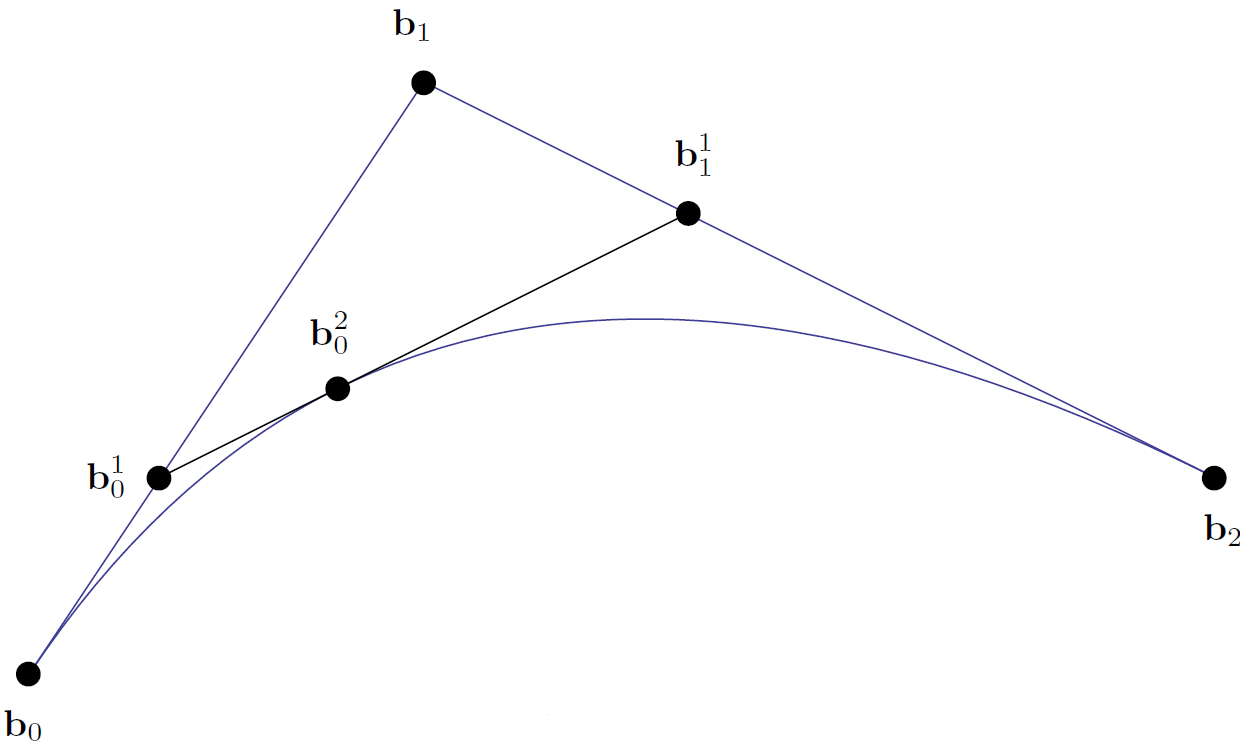
\includegraphics[width=0.275\textwidth]{images/bezier.png}
\end{center}
\begin{equation}
    \begin{tabular}{ccc}
        $b_0$ &         &         \\
        $b_1$ & $b_0^1$ &         \\
        $b_2$ & $b_1^1$ & $b_0^2$ \\
    \end{tabular}
    \nonumber
\end{equation}
Par exemple, pour les points $b_0=\binom{1}{1}, b_1=\binom{2}{\sfrac{5}{2}}, b_2=\binom{4}{\sfrac{3}{2}}$ et le pas $t=\sfrac{1}{3}$, on a:
\begin{equation}
    \begin{tabular}{ccc}
        $\begin{bmatrix}1 \\1\end{bmatrix}$            &                                                            &                                                              \\
        $\begin{bmatrix}2 \\\sfrac{5}{2}\end{bmatrix}$ & $\begin{bmatrix}\sfrac{4}{3} \\\sfrac{3}{2}\end{bmatrix}$  &                                                              \\
        $\begin{bmatrix}4 \\\sfrac{3}{2}\end{bmatrix}$ & $\begin{bmatrix}\sfrac{8}{3} \\\sfrac{13}{6}\end{bmatrix}$ & $\begin{bmatrix}\sfrac{16}{9} \\\sfrac{31}{18}\end{bmatrix}$ \\
    \end{tabular}
    \nonumber
\end{equation}
Ces points intermédiaires sont calculés comme suit:
\begin{equation}
    \begin{aligned}
         & b_0^1(t) = (1-t)\cdot b_0 + t\cdot b_1,     \\
         & b_1^1(t) = (1-t)\cdot b_1 + t\cdot b_2,     \\
         & b_0^2(t) = (1-t)\cdot b_0^1 + t\cdot b_1^1.
    \end{aligned}
    \nonumber
\end{equation}
    \columnbreak
    \subsection*{Systèmes d'équations non linéaires}
\noindent
\subsubsection*{Point fixe}
\noindent
Exemple, mettre le système suivant sous forme de point fixe :
\begin{align*}
    \left\{
    \begin{aligned}
         & x^2-10x+y^2+6 = 0 \\
         & xy^2+x-10y+5 = 0
    \end{aligned}
    \right. \\
    \overrightarrow{F}(x,y) = \begin{pmatrix} F_1(x,y) \\ F_2(x,y) \end{pmatrix} =
    \left\{
    \begin{aligned}
         & x = \frac{1}{10}\cdot (x^2+y^2+6) \\
         & y = \frac{1}{10}\cdot (xy^2+x+5)
    \end{aligned}
    \right.
\end{align*}
Et donc pour itérer :
\begin{align}
    \left\{
    \begin{aligned}
         & x_{k+1} = \frac{1}{10}\cdot (x_k^2+y_k^2+6)  \\
         & y_{k+1} = \frac{1}{10}\cdot (x_ky_k^2+x_k+5)
    \end{aligned}
    \right.
    \nonumber
\end{align}
\subsubsection*{Norme matricielle}
\noindent
\begin{equation}
    \left\|A\right\|_2 = \sqrt{a_{11}^2+a_{12}^2+\dots+a_{1n}^2+\dots+a_{n1}^2+a_{n2}^2+\dots+a_{nn}^2}
    \nonumber
\end{equation}
\subsubsection*{Matrice de Jacobi}
\noindent
\begin{equation}
    J_{\overrightarrow{F}}(x,y) =
    \begin{pmatrix}
        \frac{\partial F_1}{\partial x} & \frac{\partial F_1}{\partial y} \\
        \frac{\partial F_2}{\partial x} & \frac{\partial F_2}{\partial y}
    \end{pmatrix}
    \nonumber
\end{equation}
\subsubsection*{Contraction sur $\mathbf{D}$}
\noindent
S'il existe une constante $L<1$ telle que la norme matricielle de la matrice de Jacobi
soit inférieure à $L$ pour tout point $(x,y)\in D$, alors $\overrightarrow{F}(x,y)$ est
un contraction sur $D$ :
\begin{equation}
    J_{\overrightarrow{F}}(x,y) =
    \frac{1}{10}\cdot
    \begin{pmatrix}
        2x    & 2y        \\
        y^2+1 & 2x\cdot y
    \end{pmatrix}
    \nonumber
\end{equation}
\begin{equation}
    \left\|J_{\overrightarrow{F}}(x,y)\right\|_2 = \frac{1}{10}\cdot\sqrt{4x^2+4y^2+(y^2+1)^2+4x^2y^2}
    \nonumber
\end{equation}
sur $D=\left\{(x,y):-1\leq x\leq 1, -1\leq y\leq 1\right\}$, on a :
\begin{equation}
    \left\|J_{\overrightarrow{F}}(x,y)\right\|_2 \leq \frac{1}{10}\cdot\sqrt{4+4+4+4} = \frac{2}{5}
    \nonumber
\end{equation}
Car :
\begin{align*}
    F_1(x,y) & \leq \frac{1}{10}\cdot(1^2+1^2+6) = \frac{4}{5} < 1      \\
    F_2(x,y) & \leq \frac{1}{10}\cdot(1\cdot1^2+1+5) = \frac{7}{10} < 1
\end{align*}
\subsubsection*{Erreurs}
\noindent
Erreur a priori :
\begin{align*}
    E_k & = \frac{L^k}{1-L}\cdot\left\|\overrightarrow{F}(x_1,y_1)-\overrightarrow{F}(x_0,y_0)\right\|_2 \\
        & = \frac{L^k}{1-L}\cdot\sqrt{(x_1-x_0)^2+(y_1-y_0)^2}
    \nonumber
\end{align*}
Erreur a posteriori pour une $k^{\grave{e}me}$ itération :
\begin{align*}
    E_k & = \frac{L}{1-L}\cdot\left\|\overrightarrow{F}(x_k,y_k)-\overrightarrow{F}(x_{k-1},y_{k-1})\right\|_2 \\
        & = \frac{L}{1-L}\cdot\sqrt{(x_k-x_{k-1})^2+(y_k-y_{k-1})^2}
    \nonumber
\end{align*}
Avec $L$ la constante de Lipschitz :
\begin{equation}
    L = \max_{(x,y)\in D}\left\|J_{\overrightarrow{F}}(x,y)\right\|_2 < 1
    \nonumber
\end{equation}
\subsubsection*{Méthode de Newton (suicide)}
\noindent
\begin{equation}
    \left\{
    \begin{aligned}
         & x_{k+1} = x_k + \frac{F_2(x_k,y_k)\cdot \frac{\partial F_1(x_k, y_k)}{\partial y}-F_1(x_k,y_k)\cdot \frac{\partial F_2(x_k, y_k)}{\partial y}}{\frac{\partial F_1(x_k, y_k)}{\partial x}\cdot \frac{\partial F_2(x_k, y_k)}{\partial y}-\frac{\partial F_1(x_k, y_k)}{\partial y}\cdot \frac{\partial F_2(x_k, y_k)}{\partial x}} \\
         & y_{k+1} = y_k + \frac{F_1(x_k,y_k)\cdot \frac{\partial F_2(x_k, y_k)}{\partial x}-F_2(x_k,y_k)\cdot \frac{\partial F_1(x_k, y_k)}{\partial x}}{\frac{\partial F_1(x_k, y_k)}{\partial x}\cdot \frac{\partial F_2(x_k, y_k)}{\partial y}-\frac{\partial F_1(x_k, y_k)}{\partial y}\cdot \frac{\partial F_2(x_k, y_k)}{\partial x}}
    \end{aligned}
    \right.
    \nonumber
\end{equation}



    \subsection*{Équations non linéaires}
\noindent
\subsubsection*{Méthode de la bissection}
\noindent
On sait que le $f(x)$ coupe l'axe des $x$ entre $a$ et $b$. $a_0 = a$, $b_0 = b$
\begin{equation}
    \begin{cases}
        a_{k+1} = a_k, b_{k+1} = x_k & \text{si } f(x_k)\cdot f(a_k) < 0 \\
        a_{k+1} = x_k, b_{k+1} = b_k & \text{si } f(x_k)\cdot f(b_k) < 0 \\
        x_{k+1} = \frac{a_{k+1}+b_{k+1}}{2}
    \end{cases}
    \nonumber
\end{equation}
\subsubsection*{Méthode de la sécante}
\noindent
\begin{equation}
    x_{k+1} = x_k - \frac{f(x_k)\cdot (x_k-x_{k-1})}{f(x_k)-f(x_{k-1})}
    \nonumber
\end{equation}
\subsubsection*{Méthode de Newton}
\noindent
\begin{equation}
    x_{k+1} = x_k - \frac{f(x_k)}{f^{\prime}(x_k)}
    \nonumber
\end{equation}
\subsubsection*{Point fixe}
\noindent
Voir les autre section où on met les équations sous forme de point fixe.
\begin{equation}
    x_{k+1} = F(x_k)
    \nonumber
\end{equation}
\subsubsection*{Erreurs}
\noindent
Erreur a priori :
\begin{equation}
    E_k = \frac{L^k}{1-L}\cdot |x_1-x_0|
    \nonumber
\end{equation}
Erreur a posteriori :
\begin{equation}
    E_k = \frac{L}{1-L}\cdot |x_k-x_{k-1}|
    \nonumber
\end{equation}
Avec :
\begin{equation}
    L = \max_{x\in [a,b]}|F^{\prime}(x)| < 1
    \nonumber
\end{equation}
\subsubsection*{Vitesse de convergence}
\noindent
Plus $P$ est grand, plus la vitesse de convergence est rapide.
$r$ est la racine de $f(x)$.
\noindent
\begin{equation}
    |x_{k+1}-r| \leq C\cdot |x_k-r|^p
    \nonumber
\end{equation}


    \subsection*{Intégration numérique}
\subsubsection*{Méthode composite du trapèze}
\noindent
Pour les points $x_0, x_1, \dots, x_n$ avec $x_0=a$ et $x_n=b$.
\begin{equation}
    \left\{
    \begin{aligned}
         & T(h) = h\cdot \left[\frac{1}{2}\cdot f(a)+\sum_{j=1}^{n-1}f(x_j)+\frac{1}{2}\cdot f(b)\right] \\
         & h = \frac{b-a}{n}                                                                             \\
    \end{aligned}
    \right.
    \nonumber
\end{equation}
\subsubsection*{Méthode du point milieu}
\noindent
\begin{equation}
    \left\{
    \begin{aligned}
         & M(h) = h\cdot \sum_{j=0}^{n-1}f(x_{j+\sfrac{1}{2}}) \\
         & x_{j+\sfrac{1}{2}} = a + (j + \sfrac{1}{2})\cdot h
    \end{aligned}
    \right.
    \nonumber
\end{equation}
Il existe la relation suivant entre les deux méthodes :
\begin{equation}
    T\left(\frac{h}{2}\right) = \frac{1}{2}\cdot [T(h) + M(h)]
    \nonumber
\end{equation}
\subsubsection*{Méthode de Simpson simple}
\noindent
\begin{equation}
    S = \frac{h}{3}\cdot \left[f(a)+4\cdot f\left(\frac{a+b}{2}\right)+f(b)\right]
    \nonumber
\end{equation}
\subsubsection*{Méthode de Simpson composée}
\noindent
\begin{equation}
    \left\{
    \begin{aligned}
        S_c & = \frac{h}{3}\cdot \left(f(a)+4\cdot f(x_1)+f(b)\right.     \\
            & \quad+2\cdot \sum_{k=1}^{n-1}[f(x_{2k})+2\cdot f(x_{2k+1})] \\
        x_n & = a + n\cdot h
    \end{aligned}
    \right.
    \nonumber
\end{equation}
\subsubsection*{Méthode Newton-Cotes}
\noindent
\begin{equation}
    \left\{
    \begin{aligned}
         & Q_n=\int_a^b P_n(x)\cdot dx = \sum_{j=0}^n w_j\cdot f(x_j) \\
         & w_j = \int_a^b \prod_{\substack{k=0                        \\ k\neq j}}^n \frac{x-x_k}{x_j-x_k}\cdot dx
    \end{aligned}
    \right.
    \nonumber
\end{equation}
Exemple avec $n=1$, $x_0=a$ et $x_1=b$ parce que ça veut juste rien dire :
\begin{equation}
    Q_1 = \frac{h}{2}\cdot[f(x_0)+f(x_1)]
    \nonumber
\end{equation}
$n=2$, $x_0=a$ et $x_2=b$
\begin{equation}
    Q_2 = \frac{h}{3}\cdot[f(x_0)+4\cdot f(x_1)+f(x_2)]
    \nonumber
\end{equation}
$n=3$, $x_0=a$ et $x_3=b$
\begin{equation}
    Q_3 = \frac{3\cdot h}{8}\cdot[f(x_0)+3\cdot f(x_1)+3\cdot f(x_2)+f(x_3)]
    \nonumber
\end{equation}
$n=4$, $x_0=a$ et $x_4=b$
\begin{equation}
    Q_4 = \frac{2\cdot h}{45}\cdot[7\cdot f(x_0)+32\cdot f(x_1)+12\cdot f(x_2)+32\cdot f(x_3)+7\cdot f(x_4)]
    \nonumber
\end{equation}
\subsubsection*{Méthode de Romberg}
\noindent
Pour les $T_{i,0}$, on utilise la méthode du trapèze. Pour le reste :
\begin{equation}
    \left\{
    \begin{aligned}
         & T_{i,0} = T\left(\frac{h}{2^n}\right)                  \\
         & T_{i,j} = \frac{4^j\cdot T_{i,j-1}-T_{i-1,j-1}}{4^j-1} \\
    \end{aligned}
    \right.
    \nonumber
\end{equation}
Ce qui donne le schéma suivant :
\begin{equation}
    \begin{tabular}{ccc}
        $T_{0,0}$ &           &           \\
        $T_{1,0}$ & $T_{1,1}$ &           \\
        $T_{2,0}$ & $T_{2,1}$ & $T_{2,2}$ \\
    \end{tabular}
    \nonumber
\end{equation}
Afin d'avoir un comportement de convergence, il faut que $f(x)$ soit
$2n + 2$ fois continûment dérivable
\subsubsection*{Méthode de Gauss}
\noindent
Juste genre vraiment j'ai rien compris là.

    \subsection*{Interpolation}



    % \subsubsection*{Subsection 2}
    % \lipsum[1-10]

\end{multicols*}
\end{document}